\documentclass[a4paper, 10pt]{article}
\newcommand{\myparagraph}[1]{\paragraph{#1}\mbox{}\\}
% Packages
\usepackage[left=3cm,right=3cm, bottom=3.5cm, top=3cm]{geometry}
\usepackage{amsmath}
\usepackage[utf8]{inputenc}
\usepackage{graphicx}
\usepackage[french]{babel}
\usepackage{lastpage}
\usepackage[T1]{fontenc}
\usepackage{gensymb}
\usepackage[tight]{shorttoc}
\usepackage{tabularx}
\usepackage{wrapfig}
\usepackage{multirow}
\usepackage{float}
\usepackage{color}
\usepackage{caption}
\usepackage{wrapfig}
\usepackage{fancyhdr}
\usepackage{listings}
\usepackage{wrapfig}
%\usepackage{minted}
\usepackage{keyval}
\usepackage{kvoptions}
\usepackage{fancyvrb}
\pagestyle{fancy}
\fancyhead[L]{D. Alvarez \& L. Moos}
\fancyhead[C]{Série 2}
\fancyhead[R]{}
\fancyfoot[L]{Classe I1a}
\fancyfoot[C]{\thepage\ sur \pageref{LastPage}}
\fancyfoot[R]{HEIA}
\renewcommand{\footrulewidth}{0.5pt}

\definecolor{mygreen}{rgb}{0,0.6,0}
\definecolor{mygray}{rgb}{0.5,0.5,0.5}
\definecolor{mymauve}{rgb}{0.58,0,0.82}



\lstset{ %
  backgroundcolor=\color{white},   % choose the background color; you must add \usepackage{color} or \usepackage{xcolor}; should come as last argument
  basicstyle=\ttfamily\footnotesize,        % the size of the fonts that are used for the code
  breakatwhitespace=false,         % sets if automatic breaks should only happen at whitespace
  breaklines=true,                 % sets automatic line breaking
  captionpos=b,                    % sets the caption-position to bottom
  commentstyle=\color{mygreen},    % comment style
  deletekeywords={...},            % if you want to delete keywords from the given language
  escapeinside={\%*}{*)},          % if you want to add LaTeX within your code
  extendedchars=true,              % lets you use non-ASCII characters; for 8-bits encodings only, does not work with UTF-8
  frame=single,	                   % adds a frame around the code
  keepspaces=true,                 % keeps spaces in text, useful for keeping indentation of code (possibly needs columns=flexible)
  keywordstyle=\color{blue},       % keyword style
  language=Java,                 % the language of the code
  morekeywords={*, ...},           % if you want to add more keywords to the set
  numbers=left,                    % where to put the line-numbers; possible values are (none, left, right)
  numbersep=5pt,                   % how far the line-numbers are from the code    
  numberstyle=\tiny\color{mygray}, % the style that is used for the line-numbers
  rulecolor=\color{black},         % if not set, the frame-color may be changed on line-breaks within not-black text (e.g. comments (green here))
  showspaces=false,                % show spaces everywhere adding particular underscores; it overrides 'showstringspaces'
  showstringspaces=false,          % underline spaces within strings only
  showtabs=false,                  % show tabs within strings adding particular underscores
  stepnumber=5,                    % the step between two line-numbers. If it's 1, each line will be numbered
  firstnumber=1,  
  stringstyle=\color{mymauve},     % string literal style
  tabsize=2,	                   % sets default tabsize to 2 spaces
  title=\lstname                   % show the filename of files included with \lstinputlisting; also try caption instead of title
}

\begin{document}
\begin{titlepage}
\thispagestyle{fancy} % Cette commande permet de mettre une en-tête à la page de titre
\begin{center}

\includegraphics[width=\textwidth]{./logonb.pdf}\\
\vspace{2.5cm}
{\Huge \textbf{Série 2}}\\% Titre principal
\vspace{0.2cm}
{\huge Mine Hunt - Création d'un démineur}\\% Titre secondaire
\vspace{0.9cm}
{\LARGE David Alvarez \hspace{2cm}Luca Moos}\\% Auteurs
\vspace{0.9cm}
{\Large \today}\\
%\vspace{2 cm}
\end{center}
\vfill
\tableofcontents
\end{titlepage}
\newpage
\section{Introduction}
\subsection{Objectifs}
\begin{itemize}
\item Créer une application \emph{Java} comportant une interface utilisateur graphique
\item Réaliser une vue en créant un graphe de scène et en configurant les conteneurs et les composants
\item Insérer des images (ressources externes) dans une application
\item Structurer l'application en basant la conception et le codage sur l'architecture \emph{MVC}\footnote{Model-View-Controller}. Créer une interface du modèle permettant des variantes d'implémentation
\item Gérer les actions de l'utilisateur en traitant des événements de type \textbf{ActionEvent} et \textbf{MouseEvent}
\item Gérer un menu et créer des boîtes de dialogue simples pour informer ou questionner l'utilisateur
\end{itemize}
\section{Application}
\subsection{Vues}
\begin{minipage}{0.5\textwidth}
\subsubsection{Vue principale}
\begin{figure}[H]
\centering
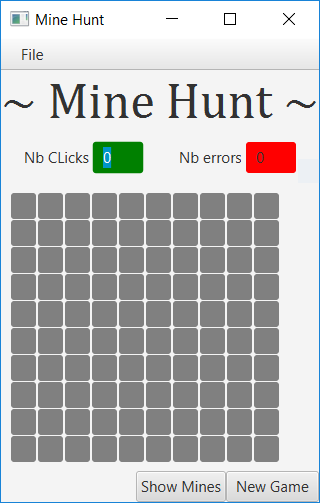
\includegraphics[]{./vprincipale.png}
\caption{Vue principale}
\end{figure}
\end{minipage}
\begin{minipage}{0.5\textwidth}
\subsubsection{Settings}
\begin{figure}[H]
\centering
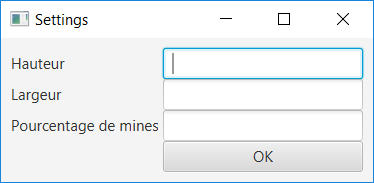
\includegraphics[]{./vsettings.png}
\caption{Vue \emph{Settings}}
\end{figure}
\end{minipage}
\subsubsection{Vue principale avec un terrain plus grand en cours de partie}
\begin{figure}[H]
\centering
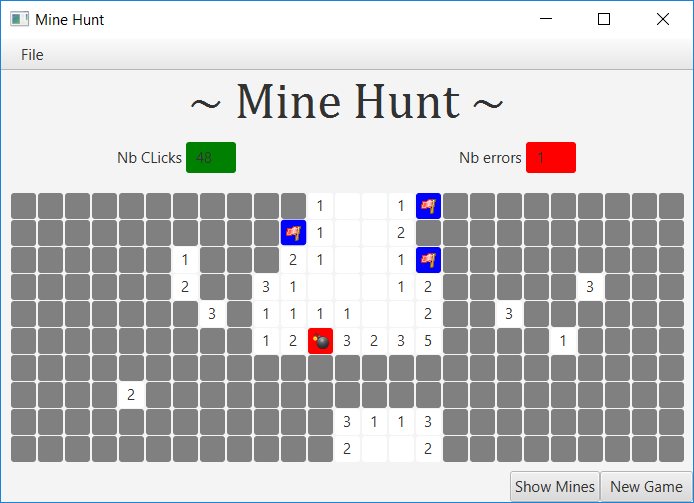
\includegraphics[]{./partie_en_cours.png}
\caption{Partie en cours}
\end{figure}
\subsection{Graphes de scène}
\subsubsection{Vue principale}
Voici le graphe de scène de la vue principale:
\begin{figure}[H]
\centering
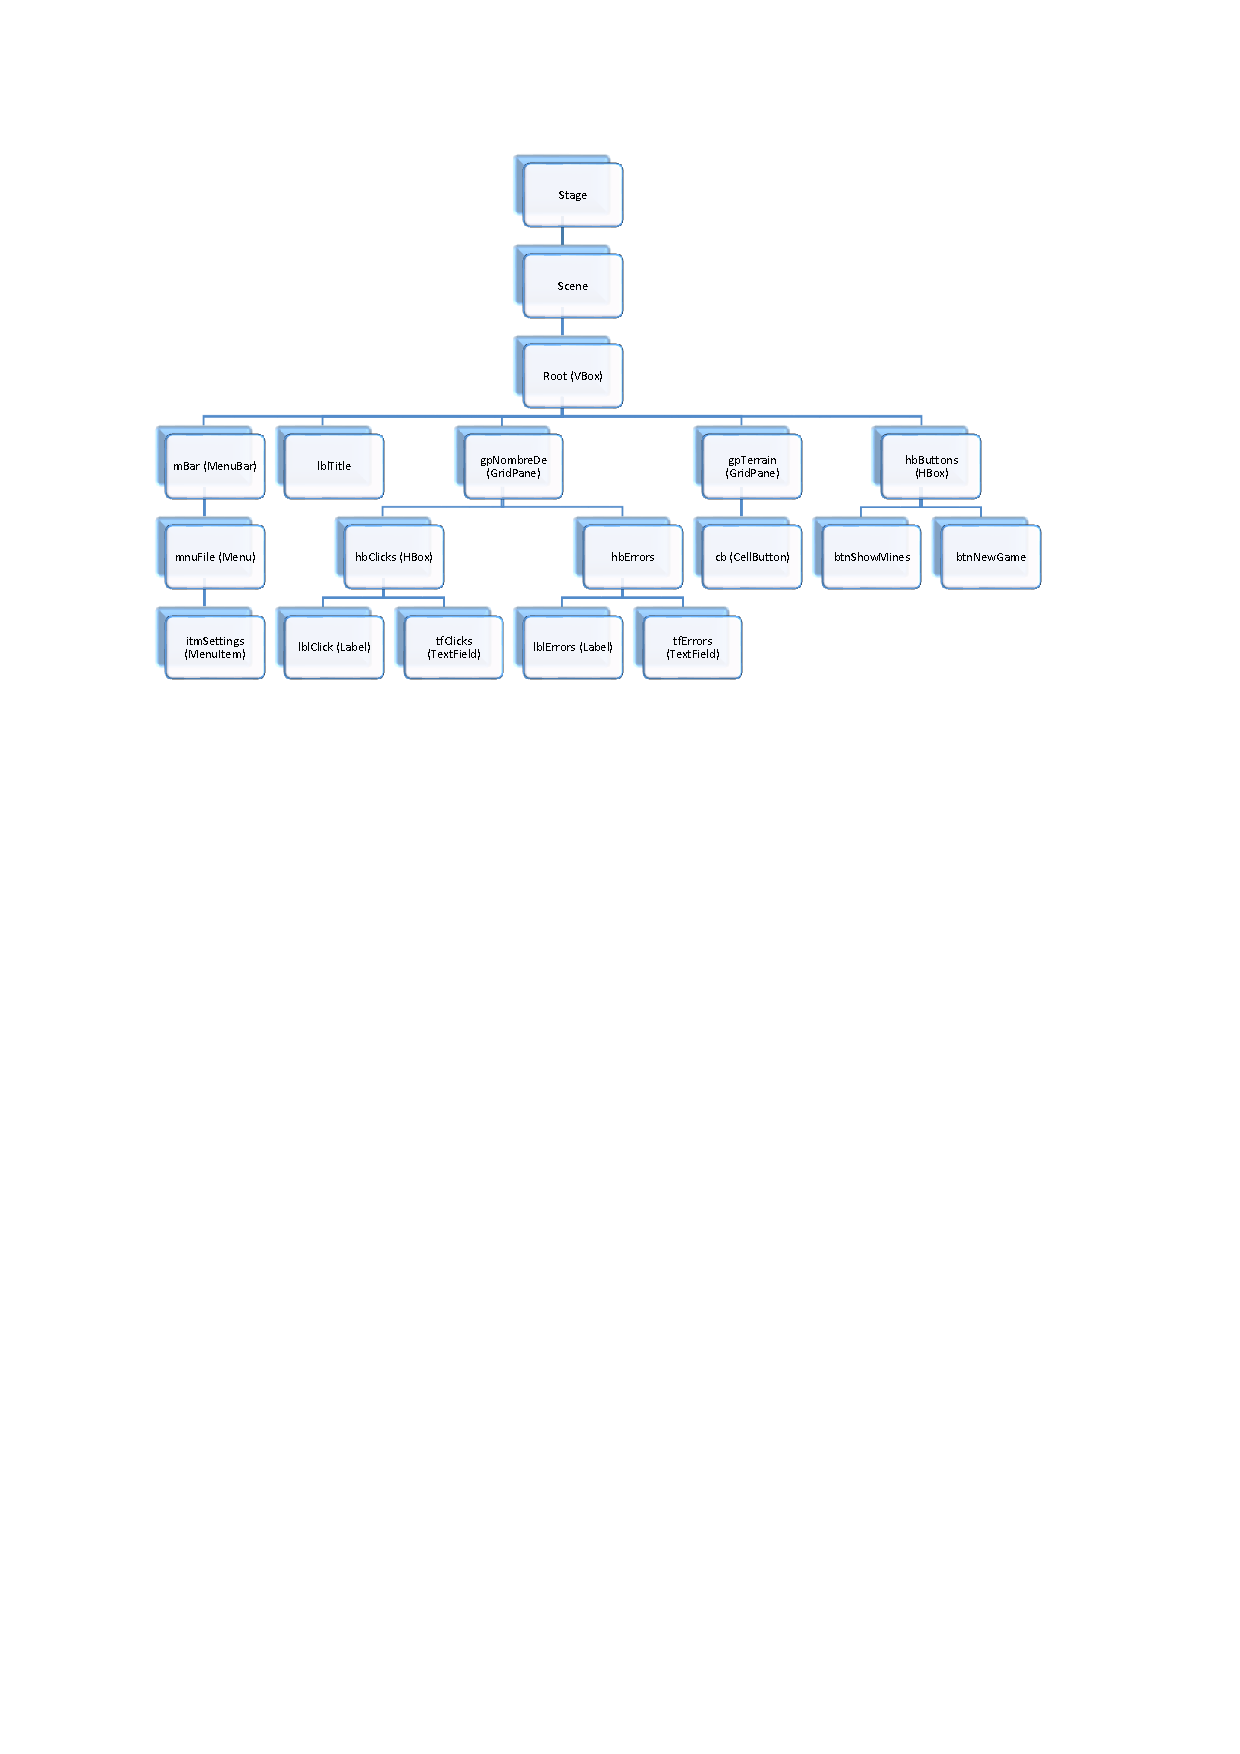
\includegraphics[width=\textwidth]{./graphe_de_scene.pdf}
\caption{Graphe de scène de la vue principale}
\end{figure}
Remarque: sur le schéma il n'y a qu'un seul \emph{cb (CellButon}. Dans la réalité, il y a $hauteur \times largeur$ nombre de \emph{Cellbuttons}.
\subsubsection{Settings}
Voici le graphe de scène de \emph{Settings}
\begin{figure}[H]
\centering
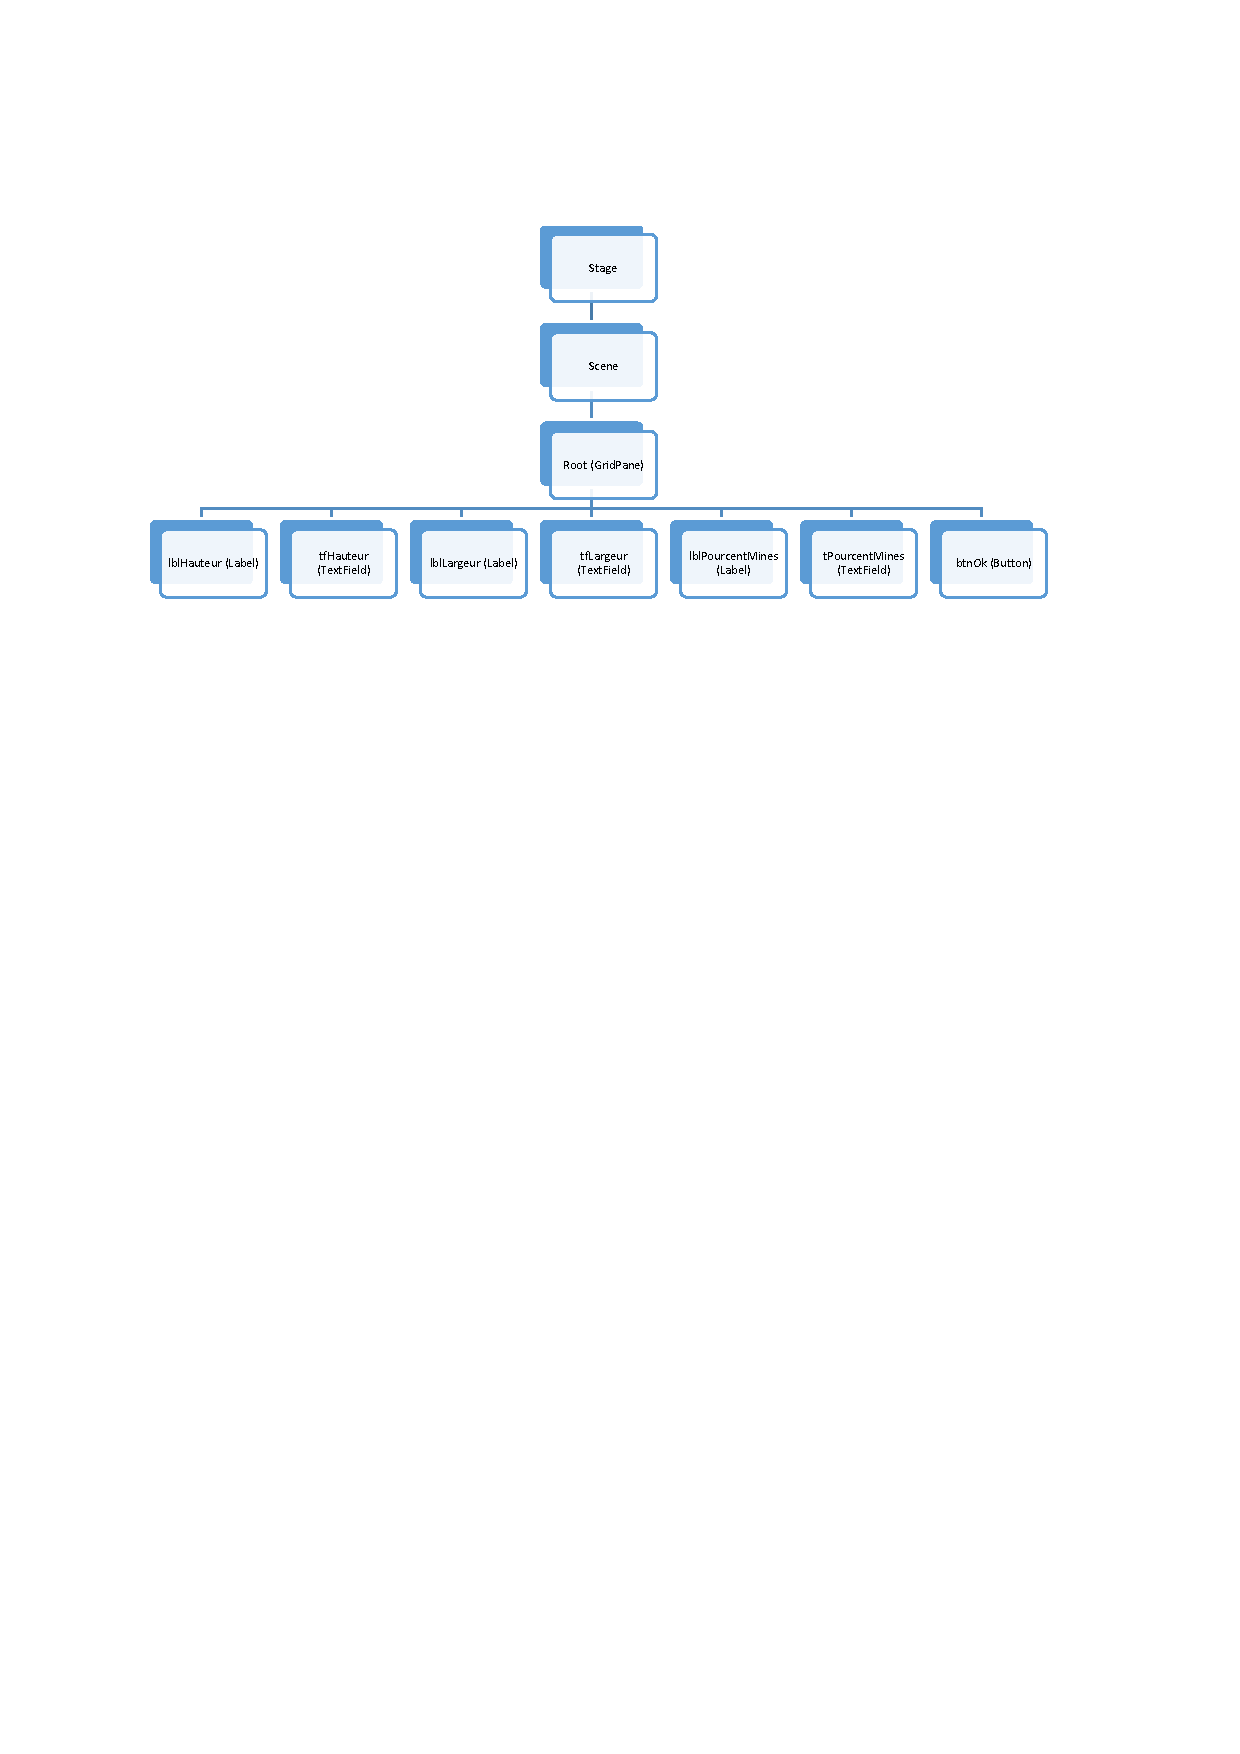
\includegraphics[width=\textwidth]{./gds_settings.pdf}
\caption{Graphe de scène de \emph{Settings}}
\end{figure}
\subsection{Description des classes}
\begin{itemize}
\item Cellbutton
\item IMineHuntModel
\item MineHuntController
\item MineHuntModel
\item MineHuntView
\item NewGameController
\item SettingController
\item SettingView
\item ShowMinesController
\item TerrainController
\end{itemize}
\vspace{0.5cm}
Et la description de chacune d'entre elles:
\begin{description}
\item[CellButton] C'est la classe que nous avons utilisée pour les mines, elle hérite de la classe \emph{Button}. Nous lui avons ajouté les attributs \emph{ligIndex} et \emph{colIndex}, afin de pouvoir savoir sur quel bouton nous cliquons (parmi tous les boutons présent dans notre "terrain" de mines
\item[IMineHuntModel] C'est l'interface de notre modèle. Elle contient les méthodes que nous pensions utiliser pour notre modèle. Finalement, notre interface ne contenait pas toutes les méthodes nécessaires, nous avons donc du en rajouter dans notre modèle
\item[MineHuntController] Cette classe permet de faire le lien entre entre la vue principale et le modèle
\item[MineHuntModel] C'est le modèle, elle contient toute l'intelligence de notre programme
\item[MineHuntView] La fenêtre principale
\item[NewGameController] Le controller faisant le lien entre le bouton \emph{New Game} et le modèle
\item[SettingController] Le controller faisant le lien entre la fenêtre \emph{Setting} et le modèle
\item[SettingView] La fenêtre secondaire permettant d'afficher les paramètre pour la partie suivante
\item[ShowMinesController] Le controller faisant le lien entre le bouton \emph{ShowMines} et le modèle
\item[TerrainController] Le controller faisant le lien entre les \emph{CellButtons} et le modèle
\end{description}
\subsection{Fonctionnalité implémentées}
Voici la liste des éléments que nous avons implémenter dans notre application :
\begin{itemize}
\item Possibilité de définir la hauteur, la largeur et le pourcentage de mines du terrain par l'utilisateur
\item Nouvelle partie
\item Montrer les mines
\item Placer des drapeaux
\item Click automatique sur toutes les cases autour d'une case n'ayant pas de mine(s) autour
\item Compteur de clicks
\item Compteur d'erreurs
\end{itemize}
\subsection{Code (fichiers \emph{.java})}
Ici, nous verrons le code de chacune des classes et expliquerons plus en détail leurs méthodes.
\subsubsection{Cellbutton.java}
\lstinputlisting[]{../CellButton.java}
\subsubsection{IMineHuntModel.java}
\lstinputlisting[]{../IMineHuntModel.java}
\subsubsection{MineHuntController.java}
\lstinputlisting[]{../MineHuntController.java}
\subsubsection{MineHuntModel.java}
Le modèle contient trois attributs principaux :
\begin{description}
\item[terrain] Tableau 2D de booléens représentant toutes les cases. \emph{true} si une bombe est présente, sinon \emph{false}
\item[dejaClique] Tableau 2D de booléens représentant l'état actuel des cases. \emph{true} si la case à déjà été cliquée, sinon \emph{false}
\item[flagged] Tableau 2D de booléens représentant les drapeaux sur le terrain. \emph{true} si un drapeau est présent sur la case, sinon \emph{false}
\end{description}
\lstinputlisting[]{../MineHuntModel.java}
\subsubsection{MineHuntView.java}
\lstinputlisting[]{../MineHuntView.java}
\subsubsection{NewGameController.java}
\lstinputlisting[]{../NewGameController.java}
\subsubsection{SettingController.java}
\lstinputlisting[]{../SettingController.java}
\subsubsection{SettingsView.java}
\lstinputlisting[]{../SettingsView.java}
\subsubsection{ShowMinesController.java}
\lstinputlisting[]{../ShowMinesController.java}
\subsubsection{TerrainController.java}
\lstinputlisting[]{../TerrainController.java}
\section{Conclusion}
Le développement de cette application fut très enrichissant. D'une part, cela nous a permis de nous familiariser avec beaucoup de composants \emph{JavaFX} et d'autre part avec l'architecture MVC et la gestion des événements.
\subsection{Difficultés rencontrées}
Voici les éléments qui nous ont posé problème:
\begin{itemize}
\item Au départ, c'était difficile de coder toutes les fonctionnalités en MVC. Nous ne pensions pas qu'il était nécessaire de mémoriser les drapeau dans le modèle par exemple. Nous étions parti sur l'idée que puisqu'il ne s'agissait que de l'affichage d'un drapeau, cela aurait pu être placé dans la vue
\item Nous sommes restés bloqués un long moment à cause des tableaux en deux dimensions. Nous en manipulons tellement, que nous avions des méthodes avec lesquelles nous prenions la hauteur à la place de la largeur et vis-versa, et cela menait à des problèmes.\\
Le simple fait que nous avons codés tout nos tableaux en mettant \emph{[ligIndex][colIndex]} nous a donné des difficultés avec l'ajout des \emph{CellButtons} dans le \emph{GridPane} parce que la méthode permettant l'ajout d'éléments dans le \emph{GridPane} prend d'abord en paramètre l'index de la colonne et ensuite l'index de la ligne. 
\end{itemize}
\subsection{Idées d'amélioration}
\begin{itemize}
\item Faire en sorte de limiter le nombre de mines pour que le programme de soit pas plus grand que l'écran
\item Dans la fenêtre \emph{Settings}, n'autoriser que les numéros dans les champs texte, ou remplacer les champs texte par des \emph{Spinners}
\item Sauvegarder la partie en cours
\end{itemize}
\end{document}